\themaG
\graphicspath{{../Ch25_La_symetrie_axiale/Images/}}

\chapter{Axes de symétrie\\et médiatrices}
\label{C21}


%%%%%%%%%%%%%%%%%%%%%%%%%%%%%%%%%%%%%%%%%%
\begin{prerequis}[Connaissances et compétences abordées]
   \begin{itemize}
      \item Axe de symétrie d’une figure, figures symétriques par rapport à un axe.
      \item Médiatrice d’un segment : définition (droite perpendiculaire au segment en son milieu) ; caractérisation (ensemble des points équidistants des extrémités du segment).
   \end{itemize}
\end{prerequis}

\vfill

\begin{debat}[Débat : mot-valise]
      Un {\bf mot-valise} est un mot formé par l'accolement du début d'un mot et la fin d'un autre mot. À l'heure actuelle, on invente régulièrement des mots-valise : {\it Brexit} pour Britain et exit, {\it Twictée} pour Twitter et dictée, {\it pourriel} pour poubelle et courriel\dots \\
      Les maths n'échappent par à la règle et le mot {\it médiatrice} est un mot-valise qui vient de médiane (dans un triangle, droite joignant un sommet au milieu du côté opposé) et bissectrice (droite coupant un angle en deux angles égaux). Il a été formé en 1923, donc très récemment.
   \begin{center}
       \begin{pspicture}(0,0)(3,3)
          \psline[linearc=0.2,linewidth=2mm,linecolor=gray](1,2)(1,2.4)(2,2.4)(2,2)
          \psframe[fillstyle=solid,fillcolor=B1,framearc=0.3](0,0)(3,2)
          \psframe[fillstyle=solid,fillcolor=A1](0.55,0)(0.85,2)
          \psarc(0.7,0.8){0.15}{180}{360}
          \psdot(0.7,0.85)
          \psframe[fillstyle=solid,fillcolor=A1](2.45,0)(2.15,2)
          \psarc(2.3,0.9){0.15}{180}{360}
          \psdot(2.3,0.95)
          \psset{linecolor=gray,linewidth=1.5mm}
          \psarc(0,0){0.3}{2}{88}
          \psarc(3,0){0.3}{92}{178}
          \psarc(3,2){0.3}{182}{268}
          \psarc(0,2){0.3}{272}{358}
       \end{pspicture}
   \end{center}
   \bigskip
   \begin{cadre}[B2][F4]
      \begin{center}
         Vidéo : \href{https://www.youtube.com/watch?v=M7npDrRJm6E}{\bf Les mots-valises}, chaîne YouTube {\it Image et communication}, épisode d'{\it Au pied de la lettre}.
      \end{center}
   \end{cadre}  
\end{debat}

\vfill

\textcolor{PartieGeometrie}{\sffamily\bfseries Cahier de compétences} : chapitre 9, exercices 1 à 10 ; 16.


%%%%%%%%%%%%%%%%%%%%%%%%%%%%%%%%%%%%
%%%%%%%%%%%%%%%%%%%%%%%%%%%%%%%%%%%%
\activites

\begin{activite}[Patchwork]
   {\bf Objectifs :} reconnaître un axe de symétrie ; suivre un programme de construction ; conjecturer une propriété.
   \begin{QCM}
      Un patchwork est une technique de couture qui consiste à assembler plusieurs morceaux de tissus de tailles, formes et couleurs différentes. \medskip
      \partie[construction de la figure]
         Construire la figure ci-dessous en suivant ce programme de construction (au crayon à papier) :
         \begin{itemize}
            \item Tracer un segment vertical $[AB]$ de longueur \ucm{8} à peu près au milieu de la feuille.
            \item Placer le milieu $O$ de ce segment.
            \item Tracer la droite $(d)$ perpendiculaire à $[AB]$ passant par $O$.
            \item Placer sur la droite $(d)$ les points $I, J, K, L$ et $M$ distants de \ucm{1,5}; \ucm{3}; \ucm{4,5}; \ucm{6} et \ucm{7,5} du point O.
            \item Joindre ces points aux extrémités du segment $[AB]$.
            \item Terminer la construction par symétrie par rapport à l’axe $(AB)$.
         \end{itemize}
         \begin{center}
            \begin{pspicture}(-4,-2.3)(4,2.3)
               \pspolygon(-3.75,0)(0,2)(3.75,0)(0,-2)
               \psset{fillstyle=solid,fillcolor=black}
               \pspolygon(2.25,0)(3,0)(0,2)
               \pspolygon(0.75,0)(1.5,0)(0,2)
               \pspolygon(0,0)(-0.75,0)(0,2)
               \pspolygon(-1.5,0)(-2.25,0)(0,2)
               \pspolygon(-3,0)(-3.75,0)(0,2)
               \pspolygon(-2.25,0)(-3,0)(0,-2)
               \pspolygon(-0.75,0)(-1.5,0)(0,-2)
               \pspolygon(0,0)(0.75,0)(0,-2)
               \pspolygon(1.5,0)(2.25,0)(0,-2)
               \pspolygon(3,0)(3.75,0)(0,-2)
            \end{pspicture}
         \end{center}
   
      \partie[analyse de la figure]
         \begin{enumerate}
            \item Que représente la droite $(d)$ pour la figure ? \\ [2mm]
               \pf
            \item Mesurer à la règle au \umm{} près les longueurs suivantes sur la figure : \bigskip
               \begin{center}
                  {\hautab{1.5}
                  \begin{tabular}{|*{5}{p{2.3cm}|}}
                     \hline
                     $IA=$ & $JA=$ & $KA=$ & $LA=$ & $MA=$ \\
                     \hline
                     $IB=$ & $JB=$ & $KB=$ & $LB=$ & $MB=$ \\
                     \hline
                  \end{tabular}}
               \end{center} \bigskip
            \item Que remarque-t-on ? \\ [2mm]
               \pf \\ [2mm]
               \pf
        \end{enumerate}

      \partie[décoration de la figure]
         Repasser les traits au stylo puis colorier la figure à votre guise. \bigskip

   \end{QCM}
   \vfill\hfill{\it\footnotesize Source : \href{http://mathsavesnes.etab.ac-lille.fr/pdf/5eme/tg2_activite_introduction_mediatrice.pdf}{mathsavesnes}, académie de Lille.}.
\end{activite}


%%%%%%%%%%%%%%%%%%%%%%%%%%%%%%%
%%%%%%%%%%%%%%%%%%%%%%%%%%%%%%%
\cours 

%%%%%%%%%%%%%%%%%%%%%%%%%%%%%%%%
\section{Axe de symétrie}

\begin{definition}
   Une figure admet un \textbf{axe de symétrique} si elle se superpose par pliage le long de cet axe.
\end{definition}

\begin{exemple*1}
   Les figures usuelles suivantes possèdent des axes de symétrie : \\
   {\psset{unit=0.6}
   \footnotesize
      \begin{pspicture}(-2,-2)(4,3)
         \pspolygon(-1,0)(1,0)(0,2)
         \psline[linecolor=B1](0,-0.5)(0,2.5)
         \rput(0,-0.9){triangle isocèle}
         \rput(0,-1.5){1 axe de symétrie}
      \end{pspicture} 
      \qquad 
      \begin{pspicture}(-2,-2)(4,3)
         \pspolygon(-1.156,0)(1.156,0)(0,2)
         \psset{linecolor=B1}
         \psline(0,-0.5)(0,2.5)
         \psline(-1.156,0)(2;50)
         \psline(1.156,0)(2;130)
          \rput(0,-0.9){triangle équilatéral}
          \rput(0,-1.5){3 axes de symétrie}
      \end{pspicture}
      \qquad
      \begin{pspicture}(-2,-2)(2,3)
         \pscircle(0,1){1}
         \psset{linecolor=B1}
         \psline(-1.5,1)(1.5,1)
         \psline(0,-0.5)(0,2.5)
         \psline(-1.5,-0.5)(1.5,2.5)
         \psline(-1.5,2.5)(1.5,-0.5)
         \psline(-0.5,-0.5)(0.5,2.5)
         \psline(-0.5,2.5)(0.5,-0.5)
         \psline(-1.5,0)(1.5,2)
         \psline(-1.5,0.5)(1.5,1.5)
         \psline(-1.5,2)(1.5,0)
         \psline(-1.5,1.5)(1.5,0.5)  
         \rput(0,-0.9){cercle} 
         \rput(0,-1.5){$\infty$ axes de symétrie}    
      \end{pspicture}

      \begin{pspicture}(-5.5,-0.9)(2,2.3)
         \psframe(-1,0)(1,2)
         \psset{linecolor= B1}
         \psline(-1.5,1)(1.5,1)
         \psline(0,-0.5)(0,2.5)
         \psline(-1.5,-0.5)(1.5,2.5)
         \psline(-1.5,2.5)(1.5,-0.5)
         \rput(0,-0.9){carré} 
         \rput(0,-1.5){4 axes de symétrie} 
      \end{pspicture}
      \qquad
      \begin{pspicture}(-4,-0.9)(2,2.3)
         \psframe(-1.5,0)(1.5,2)
         \psset{linecolor=B1}
         \psline(-2,1)(2,1)
         \psline(0,-0.5)(0,2.5)
         \rput(0,-0.9){rectangle}
         \rput(0,-1.5){2 axes de symétrie}
      \end{pspicture}
      \qquad
      \begin{pspicture}(-4,-0.9)(2,2.3)
         \pspolygon(-1.5,1)(0,0)(1.5,1)(0,2)
         \psset{linecolor= B1}
         \psline(-2,1)(2,1)
         \psline(0,-0.5)(0,2.5) 
         \rput(0,-0.9){losange}
         \rput(0,-1.5){2 axes de symétrie} 
      \end{pspicture}}
\end{exemple*1}


\section{Médiatrice} %%%%%%%%%%%%%%%%

\begin{definition}
   La \textbf{médiatrice} d'un segment est la droite qui est perpendiculaire à ce segment et qui passe par son milieu.
\end{definition}

\bigskip

Pour construire la médiatrice d'un segment, on peut utiliser la règle graduée (pour trouver le milieu du segment) et l'équerre (pour tracer la perpendiculaire à ce segment). On peut aussi utiliser le compas pour plus de précision.

\medskip

\begin{methode}[Construction de la médiatrice d'un segment à la règle et au compas]
   Pour tracer la médiatrice du segment $[AB]$, on choisit un écartement au compas et on trace deux arcs de cercle à partir de $A$ et de $B$ de part et d'autre du segment $[AB]$. \\
Puis on trace la droite passant par les deux points formés par l'intersection des arcs de cercle.
   \exercice
      {\psset{unit=0.8}
      \begin{pspicture}(-1,-0.5)(4,3.5)
         \pstGeonode[PosAngle=180,linecolor=A1](1,3){A}
          \pstGeonode[PointSymbol=none,PointName=none](0,0){C}(4,3){D}
          \pstOrtSym[linecolor=A1]{C}{D}{A}[B] 
          \pstLineAB{A}{B} 
      \end{pspicture}}
   \correction
      {\psset{unit=0.8}
      \begin{pspicture}(-1,-0.5)(4,3.5)
          \pstGeonode[PosAngle=180,linecolor=A1](1,3){A}
          \pstGeonode[PointSymbol=none,PointName=none](0,0){C}(4,3){D}
          \psarc[linecolor=A1,linestyle=dashed](1,3){2}{260}{300}
          \psarc[linecolor=A1,linestyle=dashed](1,3){2}{320}{360}
          \pstOrtSym[linecolor=A1]{C}{D}{A}[B] 
          \pstLineAB{A}{B}
          \psarc[linecolor=A1,linestyle=dashed](3.18,0.16){2}{80}{120}
          \psarc[linecolor=A1,linestyle=dashed](3.18,0.16){2}{140}{175}
      \end{pspicture} 
      \begin{pspicture}(-1,-0.5)(4,3.5)
         \pstGeonode[PosAngle=180,linecolor=A1](1,3){A}
         \pstGeonode[PointSymbol=none,PointName=none](0,0){C}(4,3){D}
         \psarc[linecolor=A1,linestyle=dashed](1,3){2}{260}{300}
         \psarc[linecolor=A1,linestyle=dashed](1,3){2}{320}{360}
         \pstOrtSym{C}{D}{A}[B] 
         \pstLineAB{A}{B}
         \psarc[linecolor=A1,linestyle=dashed](3.18,0.16){2}{80}{120}
         \psarc[linecolor=A1,linestyle=dashed](3.18,0.16){2}{140}{175}
         \pstMediatorAB[CodeFig=true,PointName=none,PointSymbol=none]{A}{B}{I}{F}  
         \pstMediatorAB[PointName=none,PointSymbol=none]{B}{A}{I}{E}     
         \pstLineAB[linecolor=B2,linewidth=0.05]{E}{F} 
      \end{pspicture}}
\end{methode}

\begin{propriete}
   \begin{itemize}
      \item Si un point appartient à la médiatrice d'un segment, alors ce point est situé à égale distance des extrémités de ce segment : on dit qu'il est \textbf{équidistant} des
extrémités du segment.
      \item Si un point est situé à égale distance des extrémités d'un segment, alors ce point appartient à la médiatrice du segment. \\ [-8mm]
   \end{itemize}
\end{propriete}

%\begin{exemple}
%   \begin{pspicture}(0,0)(5,4)
%      \pstGeonode[PosAngle={-120,60}](2,0){A}(4,3){B}
%      \pstMediatorAB[CodeFig=true,nodesep=-1.5,PosAngle={200}]{A}{B}{I}{F}
%      \psset{linecolor=teal!}
%      \psdot(4,0.83)
%      \psline{<->}(4,3)(4,0.83)
%      \psline{<->}(4,0.83)(2,0)
%      \rput(4.3,1){\textcolor{teal}{$M$}}
%      \rput{25}(3.2,0.2){\textcolor{teal}{2 cm}}
%      \rput{93}(4.3,1.9){\textcolor{teal}{2 cm}}
%      \psset{linestyle=dashed,linecolor=B1}
%      \pstSegmentMark[SegmentSymbol=MarkCros]{A}{F}
%      \pstSegmentMark[SegmentSymbol=MarkCros]{B}{F}
%   \end{pspicture}
%   \correction
%   \begin{itemize}
%      \item Les points $F$ et $I$ appartiennent à la médiatrice de $[AB]$, ils sont donc équidistants des points $A$ et $B$ : \\
%      on a $FA = FB$ et $IA =IB$.
%      \item Le point $M$ est tel que $MA = MB=2$ cm. \\
%      Il est donc situé quelque part sur la médiatrice de $[AB]$.
%   \end{itemize}
%\end{exemple}


%%%%%%%%%%%%%%%%%%%%%%%%%%%%%%%%%%%%%
%%%%%%%%%%%%%%%%%%%%%%%%%%%%%%%%%%%%%
\exercicesbase

\begin{colonne*exercice}

\serie{Axes de symétrie} %%%%%%%%%%%

\begin{exercice}
   Déterminer les axes de symétrie éventuels des lettres qui composent le mot BIJOUX.
   \begin{center}
      \begin{pspicture}(0,-0.2)(8,1.1)
         \psset{linewidth=0.1,unit=0.45}
         \psline(1.5,0)(0,0)(0,2)(1.5,2)%B
         \psline(0,1)(1.5,1)
         \psarc(1.5,0.5){0.5}{270}{90}
         \psarc(1.5,1.5){0.5}{270}{90}      
         \psline(3,0)(5,0)%I
         \psline(3,2)(5,2)
         \psline(4,0)(4,2)     
        \psline(6,2)(8,2)%J
         \psline(7,0.5)(7,2)
         \psarc(6.5,0.5){0.5}{180}{360}
         \pscircle(10,1){1}%O
         \psline(12,1)(12,2)
         \psline(14,1)(14,2)
         \psarc(13,1){1}{180}{360}
         \psline(15,0)(17,2)%X
         \psline(15,2)(17,0)      
      \end{pspicture}
   \end{center}
\end{exercice}

\begin{exercice}
   Pour chacun de ces panneaux de signalisation, tracer le ou les axes de symétrie.
   \begin{center}
   {\psset{unit=0.8}
      \begin{pspicture}(-1,-1)(2.5,1.3) %1
         \pscircle[linewidth=0.3,linecolor=red](0,0){0.85}
      \end{pspicture} 
      \begin{pspicture}(-1,-1)(2.5,1.5) %2
         \psframe[framearc=0.15](-1,-1)(1,1)
         \psframe[framearc=0.05,fillstyle=solid,fillcolor=blue,linecolor=blue](-0.9,-0.9)(0.9,0.9)
         \psframe[fillstyle=solid,fillcolor=white,linecolor=white](-0.15,-0.8)(0.15,0.3)
         \psframe[fillstyle=solid,fillcolor=white,linecolor=white](-0.4,0.3)(0.4,0.8)
         \psframe[fillstyle=solid,fillcolor=red,linecolor=red](-0.35,0.35)(0.35,0.75)
      \end{pspicture}
      \begin{pspicture}(-1,-1)(1.5,1.3) %3
         \pscircle[linewidth=0.3,linecolor=red](0,0){0.85}
         \psline[linewidth=0.2,linecolor=black](0.25,-0.55)(0.25,0.25)
         \psarc[linewidth=0.2,linecolor=black](0,0.25){0.25}{0}{180}
         \psline[linewidth=0.2,linecolor=black,arrowinset=0,arrowlength=0.5]{->}(-0.25,0.25)(-0.25,-0.4)
         \psline[linewidth=0.2,linecolor=red](1;135)(1;-45)
      \end{pspicture}   
      
      \begin{pspicture}(-1,-1)(2.5,1.5) %4
         \pspolygon[linearc=0.05,fillstyle=solid,fillcolor=white](0,-1)(1,0)(0,1)(-1,0)
         \pspolygon[linearc=0.05,fillstyle=solid,fillcolor=yellow](0,-0.68)(0.68,0)(0,0.68)(-0.68,0)
         \psline[linewidth=0.3,linecolor=black](0.7;-135)(0.7;45)
      \end{pspicture}
      \begin{pspicture}(-1,-1)(2.5,1.5) %5
         \pscircle[fillstyle=solid,fillcolor=blue,linecolor=blue](0,0){1}
         \psline[linewidth=0.2,linecolor=white](0,-0.9)(0,0.05)
         \psarc[linewidth=0.2,linecolor=white](0.4,0){0.4}{90}{180}
         \psline[linewidth=0.2,linecolor=white,arrowlength=0.8]{->}(0.35,0.4)(0.8,0.4)
         \psarc[linewidth=0.2,linecolor=white](-0.4,0){0.4}{0}{90}
         \psline[linewidth=0.2,linecolor=white,arrowlength=0.8]{->}(-0.35,0.4)(-0.8,0.4)
      \end{pspicture}
      \begin{pspicture}(-1,-1)(1.5,1.5) %6
         \psframe[framearc=0.15](-1,-1)(1,1)
         \psframe[linewidth=0.2,linecolor=blue](-0.8,-0.8)(0.8,0.8)
         \psline[linewidth=0.4,linecolor=red](0,-0.65)(0,0.65)
         \psline[linewidth=0.4,linecolor=red](-0.65,0)(0.65,0)
      \end{pspicture}
      
      \begin{pspicture}(-1,-1.5)(2.5,1.5) %7
         \pspolygon[linearc=0.05,fillstyle=solid,fillcolor=white](0,-1)(1,0)(0,1)(-1,0)
         \pspolygon[linearc=0.05,fillstyle=solid,fillcolor=yellow](0,-0.68)(0.68,0)(0,0.68)(-0.68,0)
      \end{pspicture}
      \begin{pspicture}(-1,-1.5)(2.5,1.5) %8
         \pscircle[fillstyle=solid,fillcolor=red,linecolor=red](0,0){1}
         \pscircle[fillstyle=solid,fillcolor=blue,linecolor=blue](0,0){0.7}
         \psline[linewidth=0.2,linecolor=red](1;-135)(1;45)
         \psline[linewidth=0.2,linecolor=red](1;135)(1;-45)
      \end{pspicture}
      \begin{pspicture}(-1,-1.5)(1.5,1.5) %9
         \psframe[framearc=0.15](-1,-1)(1,1)
         \psframe[framearc=0.05,fillstyle=solid,fillcolor=blue,linecolor=blue](-0.9,-0.9)(0.9,0.9)
         \pspolygon[linewidth=0.15,linecolor=orange](0.55;30)(0.55;90)(0.55;150)(0.55;210)(0.55;270)(0.55;330)
      \end{pspicture}}
   \end{center}
\end{exercice}


\serie{Médiatrice} %%%%%%%%%%%%%

\begin{exercice}
   Dans le dessin ci-dessous,
   \begin{enumerate}
      \item Quelle semble être la médiatrice du segment $[AB]$ ? $[DE]$ ? $[GH]$ ? $[AH]$ ?
      \item Quelle semble être le segment dont la médiatrice est $(d_2)$ ? $(d_3)$ ? $(d_4)$ ? $(d_8)$ ?
   \end{enumerate}
   \begin{center}
      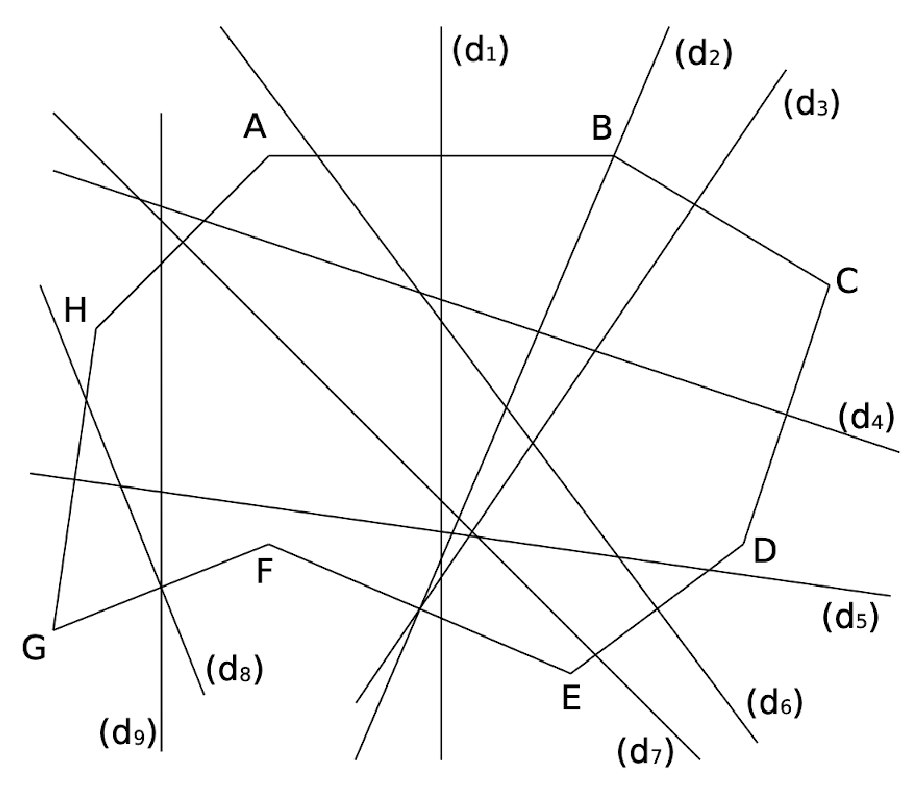
\includegraphics[width=7.5cm]{mediatrices}
   \end{center}
\end{exercice}
        
\begin{exercice}
   Construire la médiatrice de chaque segment en utilisant le quadrillage, puis coder chaque figure.
   \begin{center}
      \psset{unit=0.5}
      \begin{pspicture}(0,-3)(16,13)
         \psgrid[subgriddiv=1,linestyle=solid,gridlabels=0,gridcolor=lightgray](0,-3)(16,13)
         \psline{|-|}(1,10)(11,10)
         \psline{|-|}(1,-1)(5,3)
         \psline{|-|}(6,7)(12,1)
         \psline{|-|}(14,2)(14,10)
      \end{pspicture}
   \end{center} 
\end{exercice}

\begin{exercice}
   Tracer un triangle $NOE$ sur votre feuille de cahier.
   \begin{enumerate}
      \item Construire les médiatrices des trois côtés du triangle en utilisant la règle et l'équerre puis coder la figure.
      \item Que constate-t-on ?
      \item Tracer le cercle passant par les points $N, O$ et $E$.
   \end{enumerate}
\end{exercice}

\medskip

\begin{exercice}
   Tracer un triangle $ALI$ sur votre feuille de cahier.
   \begin{enumerate}
      \item Construire les médiatrices des trois côtés du triangle en utilisant la règle et le compas puis coder la figure.
      \item Que constate-t-on ?
      \item Tracer le cercle passant par les points $A, L$ et $I$.
   \end{enumerate}
\end{exercice}

\medskip

\begin{exercice}
   On considère le cerf-volant ci-dessous :
   \begin{center}
   \psset{unit=0.9}
      \begin{pspicture}(-1,0)(7,3.5)
         \pstGeonode[PointSymbol=none,PosAngle={180,90,0,-45}](0,0){N}(4,3){O}(6,2){U}(5,0){R}
         \pstSegmentMark{N}{O}
         \pstSegmentMark{N}{R}
         \pstSegmentMark[SegmentSymbol=MarkCros]{U}{O}
         \pstSegmentMark[SegmentSymbol=MarkCros]{U}{R}
      \end{pspicture}
   \end{center}
   \begin{enumerate}
      \item Justifier pourquoi le point $U$ appartient à la médiatrice du segment $[OR]$.
      \item Que peut-on dire des longueurs $NO$ et $NR$ ? Justifier.
      \item En déduire que les droites $(NU)$ et $(OR)$ sont perpendiculaires.
   \end{enumerate}
\end{exercice}
\hfill {\it\footnotesize Source : Les cahiers Sesamath 6\up{e}. Magnard-Sésamath 2017.}

\end{colonne*exercice}

%%%%%%%%%%%%%%%%%%%%%
%%%%%%%%%%%%%%%%%%%%%
\Recreation

\begin{activite}[Les napperons]
      Autrefois dans l'ancienne Chine, on s'offrait à l'occasion du Nouvel An chinois des sortes de \og cartes de v\oe ux \fg{} découpées dans du papier et on en décorait les murs et les portes des maisons. Pour réaliser ces cartes, on utilisait souvent le pliage et le découpage. On appelle cela des napperons.
      \partie[observation]
         Observer les napperons suivants et tracer les axes de symétrie éventuels.
         \begin{center}
            
\includegraphics[width=16cm]{napperons}
         \end{center}
         
      \partie[action !]
         Découper dans une feuille un carré de 10 cm de côté et le plier en huit comme ci-dessous (pliage rosace).
         \begin{center}
            \begin{pspicture}(-0.5,-0.1)(3.5,3)
               \rput(-0.3,1.5){1)}
               \psframe(0,0)(3,3)
               \psline[linestyle=dashed](1.5,0)(1.5,3)
               \psarc{<-}(1.5,1.5){0.75}{0}{180}
               \rput(3.3,1.5){$\Rightarrow$}
            \end{pspicture}
            \begin{pspicture}(0,0)(2,3)
               \psframe(0,0)(1.5,3)
            \end{pspicture}
            \begin{pspicture}(-0.5,0)(2,3)
               \rput(-0.3,1.5){2)}
               \psframe(0,0)(1.5,3)
               \psline[linestyle=dashed](0,1.5)(1.5,1.5)
               \psarc{->}(0.75,1.5){0.5}{90}{-90}
               \rput(1.8,0.75){$\Rightarrow$}
            \end{pspicture}
            \begin{pspicture}(0,0)(2,3)
               \psframe(0,0)(1.5,1.5)
            \end{pspicture}
            \begin{pspicture}(-0.5,0)(2,3)
               \rput(-0.3,1.5){3)}
               \psframe(0,0)(1.5,1.5)
               \psline[linestyle=dashed](0,1.5)(1.5,0)
               \psarc{->}(0.75,0.75){0.4}{45}{-135}
               \rput(1.8,0.75){$\Rightarrow$}
            \end{pspicture}
            \begin{pspicture}(0,0)(2,3)
               \pspolygon(0,0)(0,1.5)(1.5,0)
            \end{pspicture}
         \end{center}
         Découper deux figures sur les côtés du pliage obtenu puis ouvrir le napperon.
         À quoi correspondent les lignes de pli pour la figure obtenue ?
         Faire un schéma des deux napperons obtenus ci-dessous. \\ [6.7cm]
   \vfill\hfill{\it\footnotesize Source : inspiré de l'article \href{https://irem.univ-grenoble-alpes.fr/medias/fichier/68n3_1555658318837-pdf}{Le napperon, un problème pour travailler la symétrie axiale}, Grand N n\degre68, Marie-Lise Peltier, 2001}.
\end{activite}


